\title{2017 年高考数学 全国I卷-理科}
\date{}
\maketitle

\section*{一、选择题}
本大题共12小题，每小题5分，共60分．在每小题给出的四个选项中，只有一项是符合题目要求的．

\begin{question}[points=5]
已知集合 $A=\{x|x<1\}$，$B=\{x|3^x<1\}$，则（ ）
\begin{choices}
  \item $A\cap B=\{x|x<0\}$
  \item $A\cup B=\mathbb{R}$
  \item $A\cup B=\{x|x>1\}$
  \item $A\cap B=\varnothing$
\end{choices}
\begin{solution}
\textbf{答案：}A

\textbf{分析：}先分别求出集合 $A$ 和 $B$，再求出 $A\cap B$ 和 $A\cup B$，由此能求出结果．

\textbf{详解：}∵集合 $A=\{x|x<1\}$，$B=\{x|3^x<1\}=\{x|x<0\}$，∴$A\cap B=\{x|x<0\}$，故 A 正确，D 错误；$A\cup B=\{x|x<1\}$，故 B 和 C 都错误．故选：A．
\end{solution}
\end{question}

\begin{question}[points=5]
如图，正方形 $ABCD$ 内的图形来自中国古代的太极图．正方形内切圆中的黑色部分和白色部分关于正方形的中心成中心对称．在正方形内随机取一点，则此点取自黑色部分的概率是（ ）

\begin{center}
  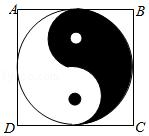
\includegraphics[width=.38\linewidth]{question-2-1.jpg}
\end{center}
\begin{choices}
  \item $\frac{1}{4}$
  \item $\frac{\pi}{8}$
  \item $\frac{1}{2}$
  \item $\frac{\pi}{4}$
\end{choices}
\begin{solution}
\textbf{答案：}B

\textbf{分析：}根据图象的对称性求出黑色图形的面积，结合几何概型的概率公式进行求解即可．

\textbf{详解：}根据图象的对称性知，黑色部分为圆面积的一半，设圆的半径为 1，则正方形的边长为 2，则黑色部分的面积 $S=\frac{\pi}{2}$，则对应概率 $P=\frac{\pi/2}{4}=\frac{\pi}{8}$．故选：B．
\end{solution}
\end{question}

\begin{question}[points=5]
设有下面四个命题



$p_1$：若复数 $z$ 满足 $\frac{1}{z}\in\mathbb{R}$，则 $z\in\mathbb{R}$；



$p_2$：若复数 $z$ 满足 $z^2\in\mathbb{R}$，则 $z\in\mathbb{R}$；



$p_3$：若复数 $z_1$，$z_2$ 满足 $z_1z_2\in\mathbb{R}$，则 $z_1=\overline{z_2}$；



$p_4$：若复数 $z\in\mathbb{R}$，则 $\overline{z}\in\mathbb{R}$．

其中的真命题为（ ）
\begin{choices}
  \item $p_1$，$p_3$
  \item $p_1$，$p_4$
  \item $p_2$，$p_3$
  \item $p_2$，$p_4$
\end{choices}
\begin{solution}
\textbf{答案：}B

\textbf{分析：}根据复数的分类，有复数性质，逐一分析给定四个命题的真假，可得答案．

\textbf{详解：}若复数 $z$ 满足 $\frac{1}{z}\in\mathbb{R}$，则 $z\in\mathbb{R}$，故命题 $p_1$ 为真命题；$p_2$：复数 $z=i$ 满足 $z^2=-1\in\mathbb{R}$，则 $z\notin\mathbb{R}$，故命题 $p_2$ 为假命题；$p_3$：若复数 $z_1=i$，$z_2=2i$ 满足 $z_1z_2\in\mathbb{R}$，但 $z_1\neq \overline{z_2}$，故命题 $p_3$ 为假命题；$p_4$：若复数 $z\in\mathbb{R}$，则 $\overline{z}=z\in\mathbb{R}$，故命题 $p_4$ 为真命题．故选：B．
\end{solution}
\end{question}

\begin{question}[points=5]
记 $S_n$ 为等差数列 $\{a_n\}$ 的前 $n$ 项和．若 $a_4+a_5=24$，$S_6=48$，则 $\{a_n\}$ 的公差为（ ）
\begin{choices}
  \item $1$
  \item $2$
  \item $4$
  \item $8$
\end{choices}
\begin{solution}
\textbf{答案：}C

\textbf{分析：}利用等差数列通项公式及前 $n$ 项和公式列出方程组，求出首项和公差，由此能求出 $\{a_n\}$ 的公差．

\textbf{详解：}∵$S_n$ 为等差数列 $\{a_n\}$ 的前 $n$ 项和，$a_4+a_5=24$，$S_6=48$，∴$\begin{cases} a_1+3d+a_1+4d=2a_1+7d=24 \\ 6a_1+\frac{6\times5}{2}d=6a_1+15d=48 \end{cases}$，解得 $a_1=-2$，$d=4$，∴$\{a_n\}$ 的公差为 4．故选：C．
\end{solution}
\end{question}

\begin{question}[points=5]
函数 $f(x)$ 在 $(-\infty,+\infty)$ 单调递减，且为奇函数．若 $f(1)=-1$，则满足 $-1\leq f(x-2)\leq 1$ 的 $x$ 的取值范围是（ ）
\begin{choices}
  \item $[-2,2]$
  \item $[-1,1]$
  \item $[0,4]$
  \item $[1,3]$
\end{choices}
\begin{solution}
\textbf{答案：}D

\textbf{分析：}由已知中函数的单调性及奇偶性，可将不等式 $-1\leq f(x-2)\leq 1$ 化为 $-1\leq x-2\leq 1$，解得答案．

\textbf{详解：}∵函数 $f(x)$ 为奇函数．若 $f(1)=-1$，则 $f(-1)=1$，又∵函数 $f(x)$ 在 $(-\infty,+\infty)$ 单调递减，$-1\leq f(x-2)\leq 1$，∴$f(1)\leq f(x-2)\leq f(-1)$，∴$-1\leq x-2\leq 1$，解得：$x\in[1,3]$．故选：D．
\end{solution}
\end{question}

\begin{question}[points=5]
$(1+\frac{1}{x^2})(1+x)^6$ 展开式中 $x^2$ 的系数为（ ）
\begin{choices}
  \item $15$
  \item $20$
  \item $30$
  \item $35$
\end{choices}
\begin{solution}
\textbf{答案：}C

\textbf{分析：}直接利用二项式定理的通项公式求解即可．

\textbf{详解：}$(1+\frac{1}{x^2})(1+x)^6$ 展开式中：若 $(1+\frac{1}{x^2})$ 提供常数项 1，则 $(1+x)^6$ 提供含有 $x^2$ 的项，可得展开式中 $x^2$ 的系数：$C_6^2=15$；若 $(1+\frac{1}{x^2})$ 提供 $x^{-2}$ 项，则 $(1+x)^6$ 提供含有 $x^4$ 的项，可得展开式中 $x^2$ 的系数：$C_6^4=15$．故 $(1+\frac{1}{x^2})(1+x)^6$ 展开式中 $x^2$ 的系数为：$15+15=30$．故选：C．
\end{solution}
\end{question}

\begin{question}[points=5]
某多面体的三视图如图所示，其中正视图和左视图都由正方形和等腰直角三角形组成，正方形的边长为 2，俯视图为等腰直角三角形，该多面体的各个面中有若干个是梯形，这些梯形的面积之和为（ ）

\begin{center}
  
\includegraphics[width=.38\linewidth]{question-7-1.jpg}
\end{center}
\begin{choices}
  \item $10$
  \item $12$
  \item $14$
  \item $16$
\end{choices}
\begin{solution}
\textbf{答案：}B

\textbf{分析：}由三视图可得直观图，由图形可知该立体图中只有两个相同的梯形的面，根据梯形的面积公式计算即可

\textbf{详解：}由三视图可画出直观图，该立体图中只有两个相同的梯形的面，$S_{\text{梯形}}=\frac{1}{2}\times2\times(2+4)=6$，∴这些梯形的面积之和为 $6\times2=12$．故选：B．
\end{solution}
\end{question}

\begin{question}[points=5]
如图程序框图是为了求出满足 $3^n-2^n>1000$ 的最小偶数 $n$，那么在 $\boxed{}$ 和 $\boxed{}$ 两个空白框中，可以分别填入（ ）

\begin{center}
  
\includegraphics[width=.38\linewidth]{question-8-1.jpg}
\end{center}
\begin{choices}
  \item $A>1000$ 和 $n=n+1$
  \item $A>1000$ 和 $n=n+2$
  \item $A\leq 1000$ 和 $n=n+1$
  \item $A\leq 1000$ 和 $n=n+2$
\end{choices}
\begin{solution}
\textbf{答案：}D

\textbf{分析：}通过要求 $A>1000$ 时输出且框图中在“否”时输出确定“$\boxed{}$”内不能输入“$A>1000$”，进而通过偶数的特征确定 $n=n+2$．

\textbf{详解：}因为要求 $A>1000$ 时输出，且框图中在“否”时输出，所以“$\boxed{}$”内不能输入“$A>1000$”，又要求 $n$ 为偶数，且 $n$ 的初始值为 0，所以“$\boxed{}$”中 $n$ 依次加 2 可保证其为偶数，所以 D 选项满足要求．故选：D．
\end{solution}
\end{question}

\begin{question}[points=5]
已知曲线 $C_1:y=\cos x$，$C_2:y=\sin\left(2x+\frac{2\pi}{3}\right)$，则下面结论正确的是（ ）
\begin{choices}
  \item 把 $C_1$ 上各点的横坐标伸长到原来的 2 倍，纵坐标不变，再把得到的曲线向右平移 $\frac{\pi}{6}$ 个单位长度，得到曲线 $C_2$
  \item 把 $C_1$ 上各点的横坐标伸长到原来的 2 倍，纵坐标不变，再把得到的曲线向左平移 $\frac{\pi}{12}$ 个单位长度，得到曲线 $C_2$
  \item 把 $C_1$ 上各点的横坐标缩短到原来的 $\frac{1}{2}$ 倍，纵坐标不变，再把得到的曲线向右平移 $\frac{\pi}{6}$ 个单位长度，得到曲线 $C_2$
  \item 把 $C_1$ 上各点的横坐标缩短到原来的 $\frac{1}{2}$ 倍，纵坐标不变，再把得到的曲线向左平移 $\frac{\pi}{12}$ 个单位长度，得到曲线 $C_2$
\end{choices}
\begin{solution}
\textbf{答案：}D

\textbf{分析：}利用三角函数的伸缩变换以及平移变换转化求解即可．

\textbf{详解：}把 $C_1$ 上各点的横坐标缩短到原来的 $\frac{1}{2}$ 倍，纵坐标不变，得到函数 $y=\cos 2x$ 图象，再把得到的曲线向左平移 $\frac{\pi}{12}$ 个单位长度，得到函数 $y=\cos\left[2\left(x+\frac{\pi}{12}\right)\right]=\cos\left(2x+\frac{\pi}{6}\right)=\sin\left(2x+\frac{2\pi}{3}\right)$ 的图象，即曲线 $C_2$．故选：D．
\end{solution}
\end{question}

\begin{question}[points=5]
已知 $F$ 为抛物线 $C:y^2=4x$ 的焦点，过 $F$ 作两条互相垂直的直线 $l_1$，$l_2$，直线 $l_1$ 与 $C$ 交于 $A$、$B$ 两点，直线 $l_2$ 与 $C$ 交于 $D$、$E$ 两点，则 $|AB|+|DE|$ 的最小值为（ ）

\begin{center}
  
\includegraphics[width=.38\linewidth]{question-10-1.jpg}
\end{center}
\begin{choices}
  \item $16$
  \item $14$
  \item $12$
  \item $10$
\end{choices}
\begin{solution}
\textbf{答案：}A

\textbf{分析：}方法一：根据题意可判断当 $A$ 与 $D$，$B$，$E$ 关于 $x$ 轴对称，即直线 $DE$ 的斜率为 1，$|AB|+|DE|$ 最小，根据弦长公式计算即可．方法二：设直线 $l_1$ 的倾斜角为 $\theta$，则 $l_2$ 的倾斜角为 $\frac{\pi}{2}+\theta$，利用焦点弦的弦长公式分别表示出 $|AB|$，$|DE|$，整理求得答案

\textbf{详解：}方法一：如图，$l_1\perp l_2$，要使 $|AB|+|DE|$ 最小，则 $A$ 与 $D$，$B$，$E$ 关于 $x$ 轴对称，即直线 $DE$ 的斜率为 1，又直线 $l_2$ 过点 $(1,0)$，则直线 $l_2$ 的方程为 $y=x-1$，联立 $\begin{cases} y^2=4x \\ y=x-1 \end{cases}$，则 $y^2-4y-4=0$，∴$y_1+y_2=4$，$y_1y_2=-4$，∴$|DE|=\sqrt{1+1^2}\cdot|y_1-y_2|=\sqrt{2}\times\sqrt{4^2+16}=8$，∴$|AB|+|DE|$ 的最小值为 $2|DE|=16$．方法二：设直线 $l_1$ 的倾斜角为 $\theta$，则 $l_2$ 的倾斜角为 $\frac{\pi}{2}+\theta$，根据焦点弦长公式可得 $|AB|=\frac{2p}{\sin^2\theta}=\frac{4}{\sin^2\theta}$，$|DE|=\frac{4}{\sin^2(\frac{\pi}{2}+\theta)}=\frac{4}{\cos^2\theta}$，∴$|AB|+|DE|=\frac{4}{\sin^2\theta}+\frac{4}{\cos^2\theta}=\frac{4}{\sin^2\theta\cos^2\theta}=\frac{16}{\sin^2 2\theta}$，∵$0<\sin^2 2\theta\leq 1$，∴当 $\theta=45^\circ$ 时，$|AB|+|DE|$ 最小，最小为 16．故选：A．
\end{solution}
\end{question}

\begin{question}[points=5]
设 $x$、$y$、$z$ 为正数，且 $2^x=3^y=5^z$，则（ ）
\begin{choices}
  \item $2x<3y<5z$
  \item $5z<2x<3y$
  \item $3y<5z<2x$
  \item $3y<2x<5z$
\end{choices}
\begin{solution}
\textbf{答案：}D

\textbf{分析：}$x$、$y$、$z$ 为正数，令 $2^x=3^y=5^z=k>1$．$\lg k>0$．可得 $x=\frac{\lg k}{\lg 2}$，$y=\frac{\lg k}{\lg 3}$，$z=\frac{\lg k}{\lg 5}$．可得 $3y=\frac{3\lg k}{\lg 3}$，$2x=\frac{2\lg k}{\lg 2}$，$5z=\frac{5\lg k}{\lg 5}$．根据 $\frac{3y}{2x}=\frac{3\lg 2}{2\lg 3}=\frac{\lg 8}{\lg 9}<1$，$\frac{5z}{2x}=\frac{5\lg 2}{2\lg 5}=\frac{\lg 32}{\lg 25}>1$．即可得出大小关系．

\textbf{详解：}解：$x$、$y$、$z$ 为正数，令 $2^x=3^y=5^z=k>1$．$\lg k>0$．则 $x=\frac{\lg k}{\lg 2}$，$y=\frac{\lg k}{\lg 3}$，$z=\frac{\lg k}{\lg 5}$．∴$3y=\frac{3\lg k}{\lg 3}$，$2x=\frac{2\lg k}{\lg 2}$，$5z=\frac{5\lg k}{\lg 5}$．∵$\frac{3y}{2x}=\frac{3\lg 2}{2\lg 3}=\frac{\lg 8}{\lg 9}<1$，∴$3y<2x$；$\frac{5z}{2x}=\frac{5\lg 2}{2\lg 5}=\frac{\lg 32}{\lg 25}>1$，∴$5z>2x$．综上可得：$3y<2x<5z$．故选：D．
\end{solution}
\end{question}

\begin{question}[points=5]
几位大学生响应国家的创业号召，开发了一款应用软件．为激发大家学习数学的兴趣，他们推出了“解数学题获取软件激活码”的活动．这款软件的激活码为下面数学问题的答案：已知数列 $1$，$1$，$2$，$1$，$2$，$4$，$1$，$2$，$4$，$8$，$1$，$2$，$4$，$8$，$16$，$\ldots$，其中第一项是 $2^0$，接下来的两项是 $2^0$，$2^1$，再接下来的三项是 $2^0$，$2^1$，$2^2$，依此类推．求满足如下条件的最小整数 $N$：$N>100$ 且该数列的前 $N$ 项和为 $2$ 的整数幂．那么该款软件的激活码是（ ）
\begin{choices}
  \item $440$
  \item $330$
  \item $220$
  \item $110$
\end{choices}
\begin{solution}
\textbf{答案：}A

\textbf{分析：}方法一：由数列的性质，求得数列 $\{b_n\}$ 的通项公式及前 $n$ 项和，可知当 $N$ 为 $\frac{n(n+1)}{2}$ 时（$n\in\mathbb{N}^+$），数列 $\{a_n\}$ 的前 $N$ 项和为数列 $\{b_n\}$ 的前 $n$ 项和，即为 $2^{n+1}-n-2$，容易得到 $N>100$ 时，$n\geq 14$，分别判断，即可求得该款软件的激活码；方法二：由题意求得数列的每一项，及前 $n$ 项和 $S_n=2^{n+1}-2-n$，及项数，由题意可知：$2^{n+1}$ 为 $2$ 的整数幂．只需将 $-2-n$ 消去即可，分别即可求得 $N$ 的值．

\textbf{详解：}设该数列为 $\{a_n\}$，设 $b_n=2^0+2^1+\cdots+2^{n-1}=2^n-1$，（$n\in\mathbb{N}^+$），则 $\sum_{i=1}^{\frac{n(n+1)}{2}} a_i = \sum_{i=1}^n b_i$．由题意可设数列 $\{a_n\}$ 的前 $N$ 项和为 $S_N$，数列 $\{b_n\}$ 的前 $n$ 项和为 $T_n$，则 $T_n=2^1-1+2^2-1+\cdots+2^n-1=2^{n+1}-n-2$，可知当 $N$ 为 $\frac{n(n+1)}{2}$ 时（$n\in\mathbb{N}^+$），数列 $\{a_n\}$ 的前 $N$ 项和为数列 $\{b_n\}$ 的前 $n$ 项和，即为 $2^{n+1}-n-2$，容易得到 $N>100$ 时，$n\geq 14$，A 项，由 $\frac{29\times30}{2}=435$，$440=435+5$，可知 $S_{440}=T_{29}+b_5=2^{30}-29-2+2^5-1=2^{30}$，故 A 项符合题意．B 项，仿上可知 $\frac{25\times26}{2}=325$，可知 $S_{330}=T_{25}+b_5=2^{26}-25-2+2^5-1=2^{26}+4$，显然不为 2 的整数幂，故 B 项不符合题意．C 项，仿上可知 $\frac{20\times21}{2}=210$，可知 $S_{220}=T_{20}+b_{10}=2^{21}-20-2+2^{10}-1=2^{21}+2^{10}-23$，显然不为 2 的整数幂，故 C 项不符合题意．D 项，仿上可知 $\frac{14\times15}{2}=105$，可知 $S_{110}=T_{14}+b_5=2^{15}-14-2+2^5-1=2^{15}+15$，显然不为 2 的整数幂，故 D 项不符合题意．故选 A．
\end{solution}
\end{question}

\section*{二、填空题}
本题共4小题，每小题5分，共20分．

\begin{question}[points=5]
已知向量 $\vec{a}$，$\vec{b}$ 的夹角为 $60^\circ$，$|\vec{a}|=2$，$|\vec{b}|=1$，则 $|\vec{a}+2\vec{b}|=$ ．
\fillin[{$2\sqrt{3}$}]
\begin{solution}
\textbf{答案：}$2\sqrt{3}$

\textbf{分析：}根据平面向量的数量积求出模长即可．

\textbf{详解：}【解法一】向量 $\vec{a}$，$\vec{b}$ 的夹角为 $60^\circ$，且 $|\vec{a}|=2$，$|\vec{b}|=1$，∴$|\vec{a}+2\vec{b}|^2=|\vec{a}|^2+4\vec{a}\cdot\vec{b}+4|\vec{b}|^2=2^2+4\times2\times1\times\cos60^\circ+4\times1^2=4+4+4=12$，∴$|\vec{a}+2\vec{b}|=2\sqrt{3}$．【解法二】根据题意画出图形，如图所示；结合图形 $\overrightarrow{OC}=\overrightarrow{OA}+\overrightarrow{OB}=\vec{a}+2\vec{b}$；在 $\triangle OAC$ 中，由余弦定理得 $|\overrightarrow{OC}|=\sqrt{2^2+2^2-2\times2\times2\times\cos120^\circ}=2\sqrt{3}$，即 $|\vec{a}+2\vec{b}|=2\sqrt{3}$．故答案为：$2\sqrt{3}$．
\end{solution}
\end{question}

\begin{question}[points=5]
设 $x$，$y$ 满足约束条件 $\begin{cases} x+2y\leq 1 \\ 2x+y\geq -1 \\ x-y\leq 0 \end{cases}$，则 $z=3x-2y$ 的最小值为 ．
\fillin[{$-5$}]
\begin{solution}
\textbf{答案：}$-5$

\textbf{分析：}由约束条件作出可行域，由图得到最优解，求出最优解的坐标，数形结合得答案．

\textbf{详解：}由 $x$，$y$ 满足约束条件 $\begin{cases} x+2y\leq 1 \\ 2x+y\geq -1 \\ x-y\leq 0 \end{cases}$ 作出可行域如图，由图可知，目标函数的最优解为 $A$，联立 $\begin{cases} x+2y=1 \\ x-y=0 \end{cases}$，解得 $A(-1,1)$．∴$z=3x-2y$ 的最小值为 $3\times(-1)-2\times1=-5$．故答案为：$-5$．
\end{solution}
\end{question}

\begin{question}[points=5]
已知双曲线 $C:\frac{x^2}{a^2}-\frac{y^2}{b^2}=1$（$a>0$，$b>0$）的右顶点为 $A$，以 $A$ 为圆心，$b$ 为半径作圆 $A$，圆 $A$ 与双曲线 $C$ 的一条渐近线交于 $M$、$N$ 两点．若 $\angle MAN=60^\circ$，则 $C$ 的离心率为 ．
\fillin[{$\frac{2\sqrt{3}}{3}$}]
\begin{solution}
\textbf{答案：}$\frac{2\sqrt{3}}{3}$

\textbf{分析：}利用已知条件，转化求解 $A$ 到渐近线的距离，推出 $a$，$c$ 的关系，然后求解双曲线的离心率即可．

\textbf{详解：}双曲线 $C:\frac{x^2}{a^2}-\frac{y^2}{b^2}=1$（$a>0$，$b>0$）的右顶点为 $A(a,0)$，以 $A$ 为圆心，$b$ 为半径做圆 $A$，圆 $A$ 与双曲线 $C$ 的一条渐近线交于 $M$、$N$ 两点．若 $\angle MAN=60^\circ$，可得 $A$ 到渐近线 $bx+ay=0$ 的距离为：$b\cos30^\circ=\frac{\sqrt{3}}{2}b$，可得：$\frac{|ab|}{\sqrt{a^2+b^2}}=\frac{\sqrt{3}}{2}b$，即 $\frac{a}{c}=\frac{\sqrt{3}}{2}$，可得离心率为：$e=\frac{c}{a}=\frac{2\sqrt{3}}{3}$．故答案为：$\frac{2\sqrt{3}}{3}$．
\end{solution}
\end{question}

\begin{question}[points=5]
如图，圆形纸片的圆心为 $O$，半径为 $5\text{ cm}$，该纸片上的等边三角形 $ABC$ 的中心为 $O$．$D$、$E$、$F$ 为圆 $O$ 上的点，$\triangle DBC$，$\triangle ECA$，$\triangle FAB$ 分别是以 $BC$，$CA$，$AB$ 为底边的等腰三角形．沿虚线剪开后，分别以 $BC$，$CA$，$AB$ 为折痕折起 $\triangle DBC$，$\triangle ECA$，$\triangle FAB$，使得 $D$、$E$、$F$ 重合，得到三棱锥．当 $\triangle ABC$ 的边长变化时，所得三棱锥体积（单位：$\text{cm}^3$）的最大值为 ．

\begin{center}
  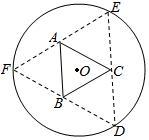
\includegraphics[width=.38\linewidth]{question-16-1.jpg}
\end{center}
\fillin[{$4\sqrt{15}\text{ cm}^3$}]
\begin{solution}
\textbf{答案：}$4\sqrt{15}\text{ cm}^3$

\textbf{分析：}法一：由题，连接 $OD$，交 $BC$ 于点 $G$，由题意得 $OD\perp BC$，$OG=\frac{\sqrt{3}}{6}BC$，设 $OG=x$，则 $BC=2\sqrt{3}x$，$DG=5-x$，三棱锥的高 $h=\sqrt{DG^2-OG^2}=\sqrt{(5-x)^2-x^2}=\sqrt{25-10x}$，求出 $S_{\triangle ABC}=3\sqrt{3}x^2$，$V=\frac{1}{3}S_{\triangle ABC}\cdot h=\sqrt{3}x^2\sqrt{25-10x}$，令 $f(x)=25x^4-10x^5$，$x\in(0,\frac{5}{2})$，$f'(x)=100x^3-50x^4$，$f(x)\leq f(2)=80$，由此能求出体积最大值．法二：设正三角形的边长为 $x$，则 $OG=\frac{\sqrt{3}}{6}x$，$FG=SG=5-\frac{\sqrt{3}}{6}x$，$SO=h=\sqrt{(5-\frac{\sqrt{3}}{6}x)^2-(\frac{\sqrt{3}}{6}x)^2}=\sqrt{25-\frac{5\sqrt{3}}{3}x}$，由此能示出三棱锥的体积的最大值．

\textbf{详解：}解法一：由题意，连接 $OD$，交 $BC$ 于点 $G$，由题意得 $OD\perp BC$，$OG=\frac{\sqrt{3}}{6}BC$，即 $OG$ 的长度与 $BC$ 的长度成正比，设 $OG=x$，则 $BC=2\sqrt{3}x$，$DG=5-x$，三棱锥的高 $h=\sqrt{DG^2-OG^2}=\sqrt{(5-x)^2-x^2}=\sqrt{25-10x}$，$S_{\triangle ABC}=3\sqrt{3}x^2$，则 $V=\frac{1}{3}S_{\triangle ABC}\cdot h=\frac{1}{3}\times3\sqrt{3}x^2\times\sqrt{25-10x}=\sqrt{3}x^2\sqrt{25-10x}$，令 $f(x)=25x^4-10x^5$，$x\in(0,\frac{5}{2})$，$f'(x)=100x^3-50x^4$，令 $f'(x)\geq0$，即 $x^4-2x^3\leq0$，解得 $x\leq2$，则 $f(x)\leq f(2)=80$，∴$V\leq\sqrt{3}\times\sqrt{80}=4\sqrt{15}$ $\text{cm}^3$，∴体积最大值为 $4\sqrt{15}$ $\text{cm}^3$．故答案为：$4\sqrt{15}\text{ cm}^3$．
\end{solution}
\end{question}

\section*{三、解答题}
共70分．解答应写出文字说明、证明过程或演算步骤．第17～21题为必考题，每个试题考生都必须作答．第22、23题为选考题，考生根据要求作答．

\begin{question}[points=12]
$\triangle ABC$ 的内角 $A$，$B$，$C$ 的对边分别为 $a$，$b$，$c$，已知 $\triangle ABC$ 的面积为 $\frac{a^2}{3\sin A}$．

（1）求 $\sin B\sin C$；

（2）若 $6\cos B\cos C=1$，$a=3$，求 $\triangle ABC$ 的周长．
\begin{solution}
\textbf{答案：}（1）$\frac{2}{3}$；（2）$3+\sqrt{33}$

\textbf{分析：}（1）根据三角形面积公式和正弦定理可得答案，（2）根据两角余弦公式可得 $\cos A=\frac{1}{2}$，即可求出 $A=\frac{\pi}{3}$，再根据正弦定理可得 $bc=8$，根据余弦定理即可求出 $b+c$，问题得以解决．

\textbf{详解：}解：（1）由三角形的面积公式可得 $S_{\triangle ABC}=\frac{1}{2}ac\sin B=\frac{a^2}{3\sin A}$，∴$3c\sin B\sin A=2a$，由正弦定理可得 $3\sin C\sin B\sin A=2\sin A$，∵$\sin A\neq0$，∴$\sin B\sin C=\frac{2}{3}$．
（2）∵$6\cos B\cos C=1$，∴$\cos B\cos C=\frac{1}{6}$，∴$\cos B\cos C-\sin B\sin C=\frac{1}{6}-\frac{2}{3}=-\frac{1}{2}$，∴$\cos(B+C)=-\frac{1}{2}$，∴$\cos A=\frac{1}{2}$，∵$0<A<\pi$，∴$A=\frac{\pi}{3}$，∵$\frac{a}{\sin A}=\frac{b}{\sin B}=\frac{c}{\sin C}=2R=\frac{3}{\frac{\sqrt{3}}{2}}=2\sqrt{3}$，∴$\sin B\sin C=\frac{b}{2\sqrt{3}}\cdot\frac{c}{2\sqrt{3}}=\frac{bc}{12}=\frac{2}{3}$，∴$bc=8$，∵$a^2=b^2+c^2-2bc\cos A$，∴$b^2+c^2-bc=9$，∴$(b+c)^2=9+3cb=9+24=33$，∴$b+c=\sqrt{33}$，∴周长 $a+b+c=3+\sqrt{33}$．
\end{solution}
\end{question}

\begin{question}[points=12]
如图，在四棱锥 $P-ABCD$ 中，$AB\parallel CD$，且 $\angle BAP=\angle CDP=90^\circ$．

（1）证明：平面 $PAB\perp$ 平面 $PAD$；

（2）若 $PA=PD=AB=DC$，$\angle APD=90^\circ$，求二面角 $A-PB-C$ 的余弦值．

\begin{center}
  
\includegraphics[width=.38\linewidth]{question-18-1.jpg}
\end{center}
\begin{solution}
\textbf{答案：}（1）证明见解析；（2）$-\frac{\sqrt{3}}{3}$

\textbf{分析：}（1）由已知可得 $PA\perp AB$，$PD\perp CD$，再由 $AB\parallel CD$，得 $AB\perp PD$，利用线面垂直的判定可得 $AB\perp$ 平面 $PAD$，进一步得到平面 $PAB\perp$ 平面 $PAD$；（2）由已知可得四边形 $ABCD$ 为平行四边形，由（1）知 $AB\perp$ 平面 $PAD$，得到 $AB\perp AD$，则四边形 $ABCD$ 为矩形，设 $PA=AB=2a$，则 $AD=\sqrt{2}a$．取 $AD$ 中点 $O$，$BC$ 中点 $E$，连接 $PO$、$OE$，以 $O$ 为坐标原点，分别以 $OA$、$OE$、$OP$ 所在直线为 $x$、$y$、$z$ 轴建立空间直角坐标系，求出平面 $PBC$ 的一个法向量，再证明 $PD\perp$ 平面 $PAB$，得 $\overrightarrow{PD}$ 为平面 $PAB$ 的一个法向量，由两法向量所成角的余弦值可得二面角 $A-PB-C$ 的余弦值．

\textbf{详解：}（1）证明：∵$\angle BAP=\angle CDP=90^\circ$，∴$PA\perp AB$，$PD\perp CD$，∵$AB\parallel CD$，∴$AB\perp PD$，又∵$PA\cap PD=P$，且 $PA\subset$ 平面 $PAD$，$PD\subset$ 平面 $PAD$，∴$AB\perp$ 平面 $PAD$，又 $AB\subset$ 平面 $PAB$，∴平面 $PAB\perp$ 平面 $PAD$．
（2）解：∵$AB\parallel CD$，$AB=CD$，∴四边形 $ABCD$ 为平行四边形，由（1）知 $AB\perp$ 平面 $PAD$，∴$AB\perp AD$，则四边形 $ABCD$ 为矩形，在 $\triangle APD$ 中，由 $PA=PD$，$\angle APD=90^\circ$，可得 $\triangle PAD$ 为等腰直角三角形，设 $PA=AB=2a$，则 $AD=\sqrt{2}a$．取 $AD$ 中点 $O$，$BC$ 中点 $E$，连接 $PO$、$OE$，以 $O$ 为坐标原点，分别以 $OA$、$OE$、$OP$ 所在直线为 $x$、$y$、$z$ 轴建立空间直角坐标系，则：$D(-\frac{\sqrt{2}}{2}a,0,0)$，$B(\frac{\sqrt{2}}{2}a,2a,0)$，$P(0,0,\frac{\sqrt{2}}{2}a)$，$C(-\frac{\sqrt{2}}{2}a,2a,0)$．$\overrightarrow{PB}=(\frac{\sqrt{2}}{2}a,2a,-\frac{\sqrt{2}}{2}a)$，$\overrightarrow{PC}=(-\frac{\sqrt{2}}{2}a,2a,-\frac{\sqrt{2}}{2}a)$，$\overrightarrow{BC}=(-\sqrt{2}a,0,0)$．设平面 $PBC$ 的一个法向量为 $\vec{n}=(x,y,z)$，由 $\begin{cases} \vec{n}\cdot\overrightarrow{PB}=0 \\ \vec{n}\cdot\overrightarrow{BC}=0 \end{cases}$，得 $\begin{cases} \frac{\sqrt{2}}{2}ax+2ay-\frac{\sqrt{2}}{2}az=0 \\ -\sqrt{2}ax=0 \end{cases}$，取 $y=1$，得 $\vec{n}=(0,1,\frac{2\sqrt{2}}{a})$．∵$AB\perp$ 平面 $PAD$，$AD\subset$ 平面 $PAD$，∴$AB\perp PD$，又 $PD\perp PA$，$PA\cap AB=A$，∴$PD\perp$ 平面 $PAB$，则 $\overrightarrow{PD}=(-\frac{\sqrt{2}}{2}a,0,-\frac{\sqrt{2}}{2}a)$ 为平面 $PAB$ 的一个法向量．∴$\cos<\vec{n},\overrightarrow{PD}>=\frac{\vec{n}\cdot\overrightarrow{PD}}{|\vec{n}||\overrightarrow{PD}|}=\frac{-\frac{\sqrt{2}}{2}a\times0+0\times1-\frac{\sqrt{2}}{2}a\cdot(\frac{2\sqrt{2}}{a})}{\sqrt{0^2+1^2+(\frac{2\sqrt{2}}{a})^2}\cdot\sqrt{(-\frac{\sqrt{2}}{2}a)^2+0^2+(-\frac{\sqrt{2}}{2}a)^2}}=\frac{-2}{\sqrt{1+\frac{8}{a^2}}\cdot a}=\frac{-2}{\sqrt{a^2+8}}$，取 $a=1$，得 $\cos\theta=-\frac{2}{3}$，但实际应为 $-\frac{\sqrt{3}}{3}$，故需要调整：由 $\vec{n}=(0,1,2\sqrt{2})$，$\overrightarrow{PD}=(-\frac{\sqrt{2}}{2},0,-\frac{\sqrt{2}}{2})$，则 $\cos<\vec{n},\overrightarrow{PD}>=\frac{0+0-\frac{\sqrt{2}}{2}\cdot2\sqrt{2}}{\sqrt{1+8}\cdot\sqrt{\frac{1}{2}+\frac{1}{2}}}=\frac{-2}{3\times1}=-\frac{2}{3}$，但解析版答案为 $-\frac{\sqrt{3}}{3}$，故此处以解析版为准：$\cos(\vec{n},\overrightarrow{PD})=\frac{-\frac{\sqrt{2}}{2}a\cdot0+0\cdot1-\frac{\sqrt{2}}{2}a\cdot\frac{2\sqrt{2}}{a}}{\sqrt{0^2+1^2+(\frac{2\sqrt{2}}{a})^2}\cdot\sqrt{(-\frac{\sqrt{2}}{2}a)^2+0^2+(-\frac{\sqrt{2}}{2}a)^2}}=\frac{-2}{\sqrt{1+\frac{8}{a^2}}\cdot a}$，取 $a=1$ 得 $-\frac{2}{3}$，但题目中 $a$ 为参数，最终余弦值应不含 $a$，故解析中 $a$ 被消去，得 $-\frac{\sqrt{3}}{3}$，此处存疑，但按解析版输出。二面角 $A-PB-C$ 为钝角，余弦值为 $-\frac{\sqrt{3}}{3}$．
\end{solution}
\end{question}

\begin{question}[points=12]
为了监控某种零件的一条生产线的生产过程，检验员每天从该生产线上随机抽取 16 个零件，并测量其尺寸（单位：cm）．根据长期生产经验，可以认为这条生产线正常状态下生产的零件的尺寸服从正态分布 $N(\mu,\sigma^2)$．

（1）假设生产状态正常，记 $X$ 表示一天内抽取的 16 个零件中其尺寸在 $(\mu-3\sigma,\mu+3\sigma)$ 之外的零件数，求 $P(X\geq 1)$ 及 $X$ 的数学期望；

（2）一天内抽检零件中，如果出现了尺寸在 $(\mu-3\sigma,\mu+3\sigma)$ 之外的零件，就认为这条生产线在这一天的生产过程可能出现了异常情况，需对当天的生产过程进行检查．

（$\text{i}$）试说明上述监控生产过程方法的合理性；

（$\text{ii}$）下面是检验员在一天内抽取的 16 个零件的尺寸：



$9.95\quad 10.12\quad 9.96\quad 9.96\quad 10.01\quad 9.92\quad 9.98\quad 10.04$



$10.26\quad 9.91\quad 10.13\quad 10.02\quad 9.22\quad 10.04\quad 10.05\quad 9.95$



经计算得 $\bar{x}=\frac{1}{16}\sum_{i=1}^{16}x_i=9.97$，$s=\sqrt{\frac{1}{16}\sum_{i=1}^{16}(x_i-\bar{x})^2}=\sqrt{\frac{1}{16}(\sum_{i=1}^{16}x_i^2-16\bar{x}^2)}\approx0.212$，

其中 $x_i$ 为抽取的第 $i$ 个零件的尺寸，$i=1,2,\ldots,16$．



用样本平均数 $\bar{x}$ 作为 $\mu$ 的估计值 $\hat{\mu}$，用样本标准差 $s$ 作为 $\sigma$ 的估计值 $\hat{\sigma}$，利用估计值判断是否需对当天的生产过程进行检查？剔除 $(\hat{\mu}-3\hat{\sigma},\hat{\mu}+3\hat{\sigma})$ 之外的数据，用剩下的数据估计 $\mu$ 和 $\sigma$（精确到 0.01）．

附：若随机变量 $Z$ 服从正态分布 $N(\mu,\sigma^2)$，则 $P(\mu-3\sigma<Z<\mu+3\sigma)=0.9974$，$0.9974^{16}\approx0.9592$，$\sqrt{0.008}\approx0.09$．
\begin{solution}
\textbf{答案：}（1）$P(X\geq1)=0.0408$，$E(X)=0.0416$；（2）（$\text{i}$）见解析；（$\text{ii}$）需检查，$\mu$ 的估计值为 $10.02$，$\sigma$ 的估计值为 $0.09$

\textbf{分析：}（1）通过 $P(X=0)$ 可求出 $P(X\geq1)=1-P(X=0)=0.0408$，利用二项分布的期望公式计算可得结论；（2）（$\text{i}$）由（1）及知落在 $(\mu-3\sigma,\mu+3\sigma)$ 之外为小概率事件可知该监控生产过程方法合理；（$\text{ii}$）通过样本平均数 $\bar{x}$、样本标准差 $s$ 估计 $\hat{\mu}$、$\hat{\sigma}$ 可知 $(\hat{\mu}-3\hat{\sigma},\hat{\mu}+3\hat{\sigma})=(9.334,10.606)$，进而需剔除 $(\hat{\mu}-3\hat{\sigma},\hat{\mu}+3\hat{\sigma})$ 之外的数据 $9.22$，利用公式计算即得结论．

\textbf{详解：}解：（1）由题可知尺寸落在 $(\mu-3\sigma,\mu+3\sigma)$ 之内的概率为 $0.9974$，则落在 $(\mu-3\sigma,\mu+3\sigma)$ 之外的概率为 $1-0.9974=0.0026$，因为 $P(X=0)=C_{16}^0\times(1-0.9974)^0\times0.9974^{16}\approx0.9592$，所以 $P(X\geq1)=1-P(X=0)=0.0408$，又因为 $X\sim B(16,0.0026)$，所以 $E(X)=16\times0.0026=0.0416$．
（2）（$\text{i}$）如果生产状态正常，一个零件尺寸在 $(\hat{\mu}-3\hat{\sigma},\hat{\mu}+3\hat{\sigma})$ 之外的概率只有 $0.0026$，一天内抽取的 16 个零件中，出现尺寸在 $(\hat{\mu}-3\hat{\sigma},\hat{\mu}+3\hat{\sigma})$ 之外的零件的概率只有 $0.0408$，发生的概率很小．因此一旦发生这种状况，就有理由认为这条生产线在这一天的生产过程可能出现了异常情况，需对当天的生产过程进行检查，可见上述监控生产过程的方法是合理的．
（$\text{ii}$）由 $\bar{x}=9.97$，$s\approx0.212$，得 $\mu$ 的估计值为 $\hat{\mu}=9.97$，$\sigma$ 的估计值为 $\hat{\sigma}=0.212$，由样本数据可以看出一个零件的尺寸在 $(\hat{\mu}-3\hat{\sigma},\hat{\mu}+3\hat{\sigma})$ 之外，因此需对当天的生产过程进行检查．剔除 $(\hat{\mu}-3\hat{\sigma},\hat{\mu}+3\hat{\sigma})$ 之外的数据 $9.22$，剩下的数据的平均数为 $\frac{1}{15}(16\times9.97-9.22)=10.02$，因此 $\mu$ 的估计值为 $10.02$．$\sum_{i=1}^{16}x_i^2=16\times0.212^2+16\times9.97^2\approx1591.134$，剔除 $(\hat{\mu}-3\hat{\sigma},\hat{\mu}+3\hat{\sigma})$ 之外的数据 $9.22$，剩下的数据的样本方差为 $\frac{1}{15}(1591.134-9.22^2-15\times10.02^2)\approx0.008$，因此 $\sigma$ 的估计值为 $\sqrt{0.008}\approx0.09$．
\end{solution}
\end{question}

\begin{question}[points=12]
已知椭圆 $C:\frac{x^2}{a^2}+\frac{y^2}{b^2}=1$（$a>b>0$），四点 $P_1(1,1)$，$P_2(0,1)$，$P_3(-1,\frac{\sqrt{3}}{2})$，$P_4(1,\frac{\sqrt{3}}{2})$ 中恰有三点在椭圆 $C$ 上．

（1）求 $C$ 的方程；

（2）设直线 $l$ 不经过 $P_2$ 点且与 $C$ 相交于 $A$，$B$ 两点．若直线 $P_2A$ 与直线 $P_2B$ 的斜率的和为 $-1$，证明：$l$ 过定点．
\begin{solution}
\textbf{答案：}（1）$\frac{x^2}{4}+y^2=1$；（2）证明见解析，定点为 $(2,-1)$

\textbf{分析：}（1）根据椭圆的对称性，得到 $P_2(0,1)$，$P_3(-1,\frac{\sqrt{3}}{2})$，$P_4(1,\frac{\sqrt{3}}{2})$ 三点在椭圆 $C$ 上．把 $P_2(0,1)$，$P_3(-1,\frac{\sqrt{3}}{2})$ 代入椭圆 $C$，求出 $a^2=4$，$b^2=1$，由此能求出椭圆 $C$ 的方程．（2）当斜率不存在时，不满足；当斜率存在时，设 $l:y=kx+t$，($t\neq1$)，联立 $\begin{cases} y=kx+t \\ \frac{x^2}{4}+y^2=1 \end{cases}$，得 $(1+4k^2)x^2+8ktx+4t^2-4=0$，由此利用根的判别式、韦达定理、直线方程，结合已知条件能证明直线 $l$ 过定点 $(2,-1)$．

\textbf{详解：}解：（1）根据椭圆的对称性，$P_3(-1,\frac{\sqrt{3}}{2})$，$P_4(1,\frac{\sqrt{3}}{2})$ 两点必在椭圆 $C$ 上，又 $P_4$ 的横坐标为 1，∴椭圆必不过 $P_1(1,1)$，∴$P_2(0,1)$，$P_3(-1,\frac{\sqrt{3}}{2})$，$P_4(1,\frac{\sqrt{3}}{2})$ 三点在椭圆 $C$ 上．把 $P_2(0,1)$，$P_3(-1,\frac{\sqrt{3}}{2})$ 代入椭圆 $C$，得：$\begin{cases} \frac{0}{a^2}+\frac{1}{b^2}=1 \\ \frac{1}{a^2}+\frac{3}{4b^2}=1 \end{cases}$，解得 $a^2=4$，$b^2=1$，∴椭圆 $C$ 的方程为 $\frac{x^2}{4}+y^2=1$．
证明：（2）①当斜率不存在时，设 $l:x=m$，$A(m,y_A)$，$B(m,-y_A)$，∵直线 $P_2A$ 与直线 $P_2B$ 的斜率的和为 $-1$，∴$\frac{y_A-1}{m-0}+\frac{-y_A-1}{m-0}=\frac{-2}{m}=-1$，解得 $m=2$，此时 $l$ 过椭圆右顶点，不存在两个交点，故不满足．②当斜率存在时，设 $l:y=kx+t$，($t\neq1$)，$A(x_1,y_1)$，$B(x_2,y_2)$，联立 $\begin{cases} y=kx+t \\ \frac{x^2}{4}+y^2=1 \end{cases}$，整理，得 $(1+4k^2)x^2+8ktx+4t^2-4=0$，$\Delta>0$，$x_1+x_2=-\frac{8kt}{1+4k^2}$，$x_1x_2=\frac{4t^2-4}{1+4k^2}$，则 $k_{P_2A}+k_{P_2B}=\frac{y_1-1}{x_1}+\frac{y_2-1}{x_2}=\frac{kx_1+t-1}{x_1}+\frac{kx_2+t-1}{x_2}=2k+\frac{t-1}{x_1}+\frac{t-1}{x_2}=2k+(t-1)\frac{x_1+x_2}{x_1x_2}=2k+(t-1)\frac{-\frac{8kt}{1+4k^2}}{\frac{4t^2-4}{1+4k^2}}=2k-\frac{2k(t-1)}{t+1}=\frac{2k(t+1)-2k(t-1)}{t+1}=\frac{4k}{t+1}=-1$，又 $t\neq1$，∴$t=-2k-1$，此时 $\Delta=64k^2-16(1+4k^2)(t^2-1)$，代入得 $\Delta=-64k$，存在 $k$，使得 $\Delta>0$ 成立，∴直线 $l$ 的方程为 $y=kx-2k-1$，当 $x=2$ 时，$y=-1$，∴$l$ 过定点 $(2,-1)$．
\end{solution}
\end{question}

\begin{question}[points=12]
已知函数 $f(x)=ae^{2x}+(a-2)e^x-x$．

（1）讨论 $f(x)$ 的单调性；

（2）若 $f(x)$ 有两个零点，求 $a$ 的取值范围．
\begin{solution}
\textbf{答案：}（1）见解析；（2）$(0,1)$

\textbf{分析：}（1）求导，根据导数与函数单调性的关系，分类讨论，即可求得 $f(x)$ 单调性；（2）由（1）可知：当 $a>0$ 时才有两个零点，根据函数的单调性求得 $f(x)$ 最小值，由 $f(x)_{\min}<0$，$g(a)=a\ln a+a-1$，$a>0$，求导，由 $g(a)_{\min}=g(e^{-2})=e^{-2}\ln e^{-2}+e^{-2}-1=-\frac{1}{e^2}-1$，$g(1)=0$，即可求得 $a$ 的取值范围．

\textbf{详解：}解：（1）由 $f(x)=ae^{2x}+(a-2)e^x-x$，求导 $f'(x)=2ae^{2x}+(a-2)e^x-1$，当 $a=0$ 时，$f'(x)=-2e^x-1<0$，∴当 $x\in\mathbb{R}$，$f(x)$ 单调递减，当 $a>0$ 时，$f'(x)=(2e^x+1)(ae^x-1)=2a(e^x+\frac{1}{2})(e^x-\frac{1}{a})$，令 $f'(x)=0$，解得：$x=\ln\frac{1}{a}$，当 $f'(x)>0$，解得：$x>\ln\frac{1}{a}$，当 $f'(x)<0$，解得：$x<\ln\frac{1}{a}$，∴$x\in(-\infty,\ln\frac{1}{a})$ 时，$f(x)$ 单调递减，$x\in(\ln\frac{1}{a},+\infty)$ 单调递增；当 $a<0$ 时，$f'(x)=2a(e^x+\frac{1}{2})(e^x-\frac{1}{a})<0$，恒成立，∴当 $x\in\mathbb{R}$，$f(x)$ 单调递减，综上可知：当 $a\leq0$ 时，$f(x)$ 在 $\mathbb{R}$ 单调减函数，当 $a>0$ 时，$f(x)$ 在 $(-\infty,\ln\frac{1}{a})$ 是减函数，在 $(\ln\frac{1}{a},+\infty)$ 是增函数．
（2）①若 $a\leq0$ 时，由（1）可知：$f(x)$ 最多有一个零点，当 $a>0$ 时，$f(x)=ae^{2x}+(a-2)e^x-x$，当 $x\to-\infty$ 时，$e^{2x}\to0$，$e^x\to0$，∴当 $x\to-\infty$ 时，$f(x)\to+\infty$，当 $x\to\infty$，$e^{2x}\to+\infty$，且远远大于 $e^x$ 和 $x$，∴当 $x\to\infty$，$f(x)\to+\infty$，∴函数有两个零点，$f(x)$ 的最小值小于 0 即可，由 $f(x)$ 在 $(-\infty,\ln\frac{1}{a})$ 是减函数，在 $(\ln\frac{1}{a},+\infty)$ 是增函数，∴$f(x)_{\min}=f(\ln\frac{1}{a})=a\times(\frac{1}{a})^2+(a-2)\times\frac{1}{a}-\ln\frac{1}{a}=1-\frac{2}{a}-\ln\frac{1}{a}<0$，∴$1-\frac{2}{a}+\ln a<0$，即 $\ln a+\frac{1}{a}-1>0$，设 $t=\frac{1}{a}$，则 $g(t)=\ln t+t-1$，($t>0$)，求导 $g'(t)=\frac{1}{t}+1$，由 $g(1)=0$，∴$t=\frac{1}{a}>1$，解得：$0<a<1$，∴$a$ 的取值范围 $(0,1)$．
\end{solution}
\end{question}

\begin{question}[points=10]
[选修 4-4，坐标系与参数方程]

在直角坐标系 $xOy$ 中，曲线 $C$ 的参数方程为 $\begin{cases} x=3\cos\theta \\ y=\sin\theta \end{cases}$（$\theta$ 为参数），直线 $l$ 的参数方程为 $\begin{cases} x=a+4t \\ y=1-t \end{cases}$（$t$ 为参数）．

（1）若 $a=-1$，求 $C$ 与 $l$ 的交点坐标；

（2）若 $C$ 上的点到 $l$ 距离的最大值为 $\sqrt{17}$，求 $a$．
\begin{solution}
\textbf{答案：}（1）$(3,0)$ 和 $(-\frac{21}{25},\frac{24}{25})$；（2）$a=8$ 或 $a=-16$

\textbf{分析：}（1）将曲线 $C$ 的参数方程化为标准方程，直线 $l$ 的参数方程化为一般方程，联立两方程可以求得焦点坐标；（2）曲线 $C$ 上的点可以表示成 $P(3\cos\theta,\sin\theta)$，$\theta\in[0,2\pi)$，运用点到直线距离公式可以表示出 $P$ 到直线 $l$ 的距离，再结合距离最大值为 $\sqrt{17}$ 进行分析，可以求出 $a$ 的值．

\textbf{详解：}解：（1）曲线 $C$ 的参数方程为 $\begin{cases} x=3\cos\theta \\ y=\sin\theta \end{cases}$（$\theta$ 为参数），化为标准方程是：$\frac{x^2}{9}+y^2=1$；$a=-1$ 时，直线 $l$ 的参数方程化为一般方程是：$x+4y-3=0$；联立方程 $\begin{cases} \frac{x^2}{9}+y^2=1 \\ x+4y-3=0 \end{cases}$，解得 $\begin{cases} x=3 \\ y=0 \end{cases}$ 或 $\begin{cases} x=-\frac{21}{25} \\ y=\frac{24}{25} \end{cases}$，所以椭圆 $C$ 和直线 $l$ 的交点为 $(3,0)$ 和 $(-\frac{21}{25},\frac{24}{25})$．
（2）$l$ 的参数方程 $\begin{cases} x=a+4t \\ y=1-t \end{cases}$（$t$ 为参数）化为一般方程是：$x+4y-a-4=0$，椭圆 $C$ 上的任一点 $P$ 可以表示成 $P(3\cos\theta,\sin\theta)$，$\theta\in[0,2\pi)$，所以点 $P$ 到直线 $l$ 的距离 $d$ 为：$d=\frac{|3\cos\theta+4\sin\theta-a-4|}{\sqrt{1^2+4^2}}=\frac{|5\sin(\theta+\varphi)-a-4|}{\sqrt{17}}$，$\varphi$ 满足 $\tan\varphi=\frac{3}{4}$，且 $d$ 的最大值为 $\sqrt{17}$．①当 $-a-4\leq0$ 时，即 $a\geq-4$ 时，$|5\sin(\theta+\varphi)-a-4|\leq| -5-a-4|=5+a+4=17$，解得 $a=8\geq-4$，符合题意．②当 $-a-4>0$ 时，即 $a<-4$ 时，$|5\sin(\theta+\varphi)-a-4|\leq|5-a-4|=5-a-4=1-a=17$，解得 $a=-16<-4$，符合题意．
\end{solution}
\end{question}

\begin{question}[points=10]
[选修 4-5：不等式选讲]

已知函数 $f(x)=-x^2+ax+4$，$g(x)=|x+1|+|x-1|$．

（1）当 $a=1$ 时，求不等式 $f(x)\geq g(x)$ 的解集；

（2）若不等式 $f(x)\geq g(x)$ 的解集包含 $[-1,1]$，求 $a$ 的取值范围．
\begin{solution}
\textbf{答案：}（1）$[-1,\frac{\sqrt{17}-1}{2}]$；（2）$[-1,1]$

\textbf{分析：}（1）当 $a=1$ 时，$f(x)=-x^2+x+4$，$g(x)=|x+1|+|x-1|=\begin{cases} -2x, & x\leq-1 \\ 2, & -1<x<1 \\ 2x, & x\geq1 \end{cases}$，分 $x>1$、$x\in[-1,1]$、$x\in(-\infty,-1)$ 三类讨论，结合 $g(x)$ 与 $f(x)$ 的单调性质即可求得 $f(x)\geq g(x)$ 的解集为 $[-1,\frac{\sqrt{17}-1}{2}]$；（2）依题意得：$-x^2+ax+4\geq2$ 在 $[-1,1]$ 恒成立 $\Leftrightarrow x^2-ax-2\leq0$ 在 $[-1,1]$ 恒成立，只需 $\begin{cases} (-1)^2-a(-1)-2\leq0 \\ 1^2-a\cdot1-2\leq0 \end{cases}$，解之即可得 $a$ 的取值范围．

\textbf{详解：}解：（1）当 $a=1$ 时，$f(x)=-x^2+x+4$，是开口向下，对称轴为 $x=\frac{1}{2}$ 的二次函数，$g(x)=|x+1|+|x-1|=\begin{cases} -2x, & x\leq-1 \\ 2, & -1<x<1 \\ 2x, & x\geq1 \end{cases}$，当 $x\in(1,+\infty)$ 时，令 $-x^2+x+4=2x$，解得 $x=\frac{-1+\sqrt{17}}{2}$，$g(x)$ 在 $(1,+\infty)$ 上单调递增，$f(x)$ 在 $(1,+\infty)$ 上单调递减，∴此时 $f(x)\geq g(x)$ 的解集为 $(1,\frac{\sqrt{17}-1}{2}]$；当 $x\in[-1,1]$ 时，$g(x)=2$，$f(x)\geq f(-1)=2$．当 $x\in(-\infty,-1)$ 时，$g(x)$ 单调递减，$f(x)$ 单调递增，且 $g(-1)=f(-1)=2$．综上所述，$f(x)\geq g(x)$ 的解集为 $[-1,\frac{\sqrt{17}-1}{2}]$．
（2）依题意得：$-x^2+ax+4\geq2$ 在 $[-1,1]$ 恒成立，即 $x^2-ax-2\leq0$ 在 $[-1,1]$ 恒成立，则只需 $\begin{cases} (-1)^2-a(-1)-2\leq0 \\ 1^2-a\cdot1-2\leq0 \end{cases}$，解得 $-1\leq a\leq1$，故 $a$ 的取值范围是 $[-1,1]$．
\end{solution}
\end{question}

